\graphicspath{{chapters/images/08/}}

\chapter{Shotgun Metagenomics}

\section{Introduction}

    \subsection{Shotgun metagenomic analysis}
    A shotgun metagenomic analysis consists of different steps:

    \begin{multicols}{2}
        \begin{itemize}
            \item Experimental pipeline: from sample collection to DNA sequencing.
            \item Preprocessing:  decontamination and quality control.
            \item Mapping, assembling or both.
            \item Sequence analysis:  identification of microbial species and identification of present pathways and functions.
            \item Post Processing: integrate data with other information coming from sample metadata.
            \item Validation:  follow-up experiments with independent replicates.
        \end{itemize}
    \end{multicols}

    \begin{figure}[!h]
        \centering
        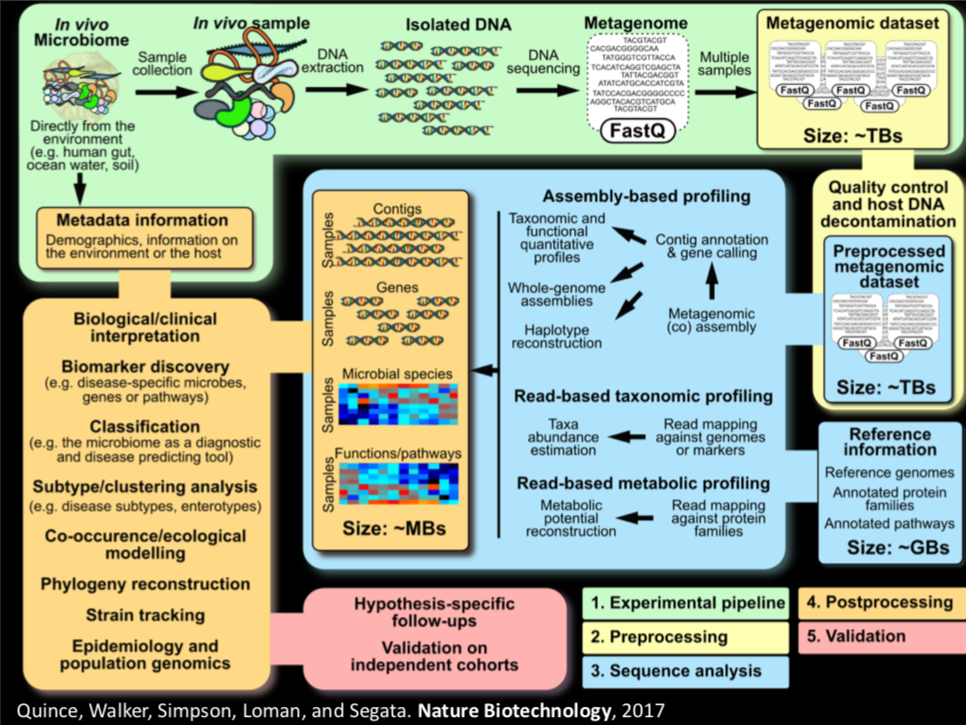
\includegraphics[width=0.9\textwidth]{Shotgun_workflow.png}
        \caption{\label{fig:workflow}Shotgun metagenomics workflow}
    \end{figure}

    \subsection{Comparison with the 16s sequencing}

    \begin{tabular}{ | m{7cm}| m{7cm} | }
     \hline
     \multicolumn{2}{|c|}{16S sequencing} \\
     \hline
     Pros & Cons \\
     \hline
     Cost-effective & Non genome-wide \\
     Avoids non-bacterial contamination & Limited taxonomic resolution \\
     Can catch low-abundance bacteria & Not useful for pathogens profiling \\
     The output has reasonable size and complexity & Does not detect viruses or eukaryotes \\
     Mature software available to perform the computations & Several biases\\
     & Cross studies are difficult: the comparison is not possible due to biases \\
     \hline\hline
     \multicolumn{2}{|c|}{Shotgun sequencing} \\
     \hline
     Pros & Cons \\
     \hline
     Genome-wide: it is possible to retrieve information about all the genes present in the metagenome & Expensive (but costs are decreasing: right now the cost for the sequencing of one sample is $\sim100\$$) \\
     High taxonomic resolution & DNA contamination are hard to remove \\
     Easy cross-study comparison thanks to the lack of biases & Low-abundance bacteria could be missed \\
     All domains of life can potentially be observed in the same study & Large dataset as output, that can be difficult to process (TBs of data) \\
     \hline
    \end{tabular}

    \subsection{Latest technology}
    The cost of $100\$$ for the sequencing of one sample refers to a sample size of $5Gb$, that should be enough for shotgun metagenomics.
    More sequencing depth could be needed if microbes with very low abundances needs to be detected, if many new genomes need to be assembled or if there is a lot of contamination.
    Shotgun metagenomics is possible with Illumina Hiseq technology, but the latest and most used technology nowadays is Illumina NovaSeq.

\section{Identification of microbes from Shotgun metagenomics data}
The main challenges with respect to identifying microbes from metagenomics data are:

\begin{multicols}{2}
    \begin{itemize}
        \item How to obtain species-specific resolution.
        \item Computational feasibility.
        \item Being able to detect both bacteria and archaea.
            Phages are also a problem since there is little reference.
        \item Obtain relative abundances of organisms with different genome sizes.
        \item Consistent detection confidence for all clades.
        \item How to handle reads as short as $50nts$.
        \item Detect organisms without a sequenced genome or still unknown species.
    \end{itemize}
\end{multicols}

    \subsection{MetaPhlAn: unique marker genes for taxonomic profiling}
    The main idea of MetaPhlAn is to find a marker gene that uniquely characterizes a species.
    This gene has to be present in all strains of a species and in no other species.
    This markers form taxonomic clades.
    ChocoPhlAn is the tool that generates the database necessary.
    From a number of genomes, ChocoPhlAn was used to create a database of marker genes that build the MetaPhlAn database.
    This database contains $200$ markers per species and its reduced dimension with respect to the whole genomes database can align reads directly to the marker database.

    \begin{figure}[!h]
        \centering
        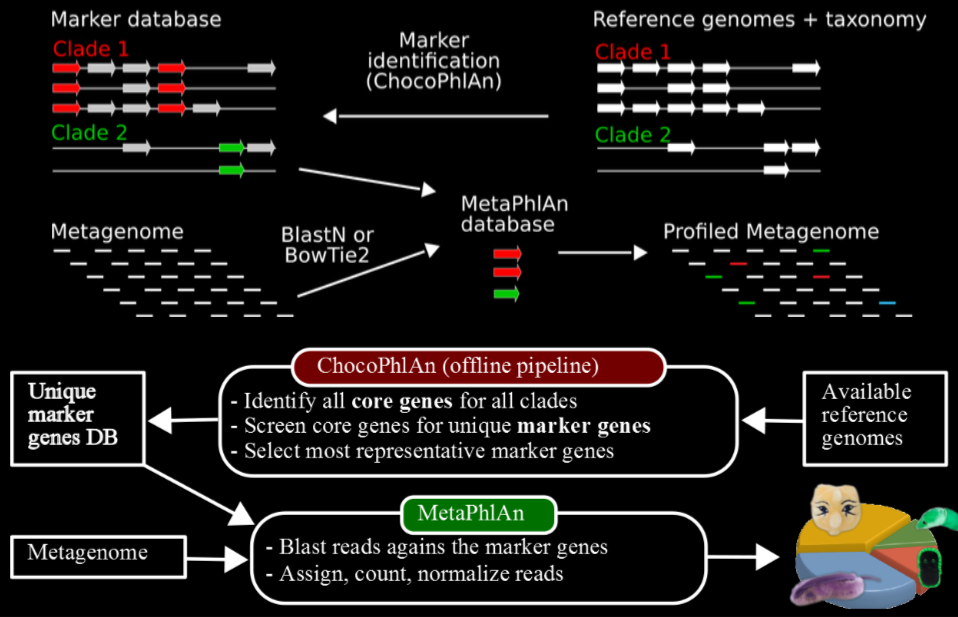
\includegraphics[width=0.95\textwidth]{MetaPhlAn.png}
        \caption{\label{fig:metaphlan}MetaPhlAn overview}
    \end{figure}


        \subsubsection{Creation of the marker genes database}
        The marker database was created from $2887$ genomes from $1222$ species.
        The number of marker per species decreases with more sequenced genomes because the core genome tends to become smaller in size and noise is eliminated.
        In the current version $1$ milion genomes are considered, with $200000$ isolated genomes and $800000$ from metagenomics assembled genomes or MAGs.

        \subsubsection{Efficiency and validation}
        MetaPhlAn can deal with $200000$ reads per second and can profile thousands of microbiomes in a few hours.
        Validation can be done with synthetic metagenomes created with errors or with biological methods: comparing the results with the ones obtained with 16S based abundance estimations.

        \subsubsection{The problem of the unknowns}
        Microbial species that were never observed and do not have a marker in the database cannot be detected with this method.
        A possible solution is to cluster together contigs obtained from the metagenome based on coverage, GC content, codon bias, and other possible features.
        Strict quality controls are then performed on these putative genomes: on the number of genes and the number of known single-copy genes in order to be sure that what has been found is not a mixture of genomes.
        High quality putative genomes are considered MAGs and version 4 of MetaPhlAn can include them in the creation of the marker database.
        This way, these species can be detected in metagenomes even though they do not have a name yet.

    \subsection{Other approaches}
    Other approaches include:

    \begin{multicols}{2}
        \begin{itemize}
            \item Sequence-based clustering of contigs to create putative genomes.
                The output are unlabelled bins with relative abundances.
                The main problem is that high coverage is needed to obtain valid results.
            \item Machine learning algorithms that exploit GC content (and possibly other features) to give as output clades with relative abundances.
                This method is not completely reference-free as it uses reference genomes to extract the features used for the classification.
                The main problem is that many species could have really similar features.
            \item Read-to-genome sequence mapping.
                In this approach there is no processing of a reference genome.
        \end{itemize}
    \end{multicols}

    \begin{figure}[H]
        \centering
        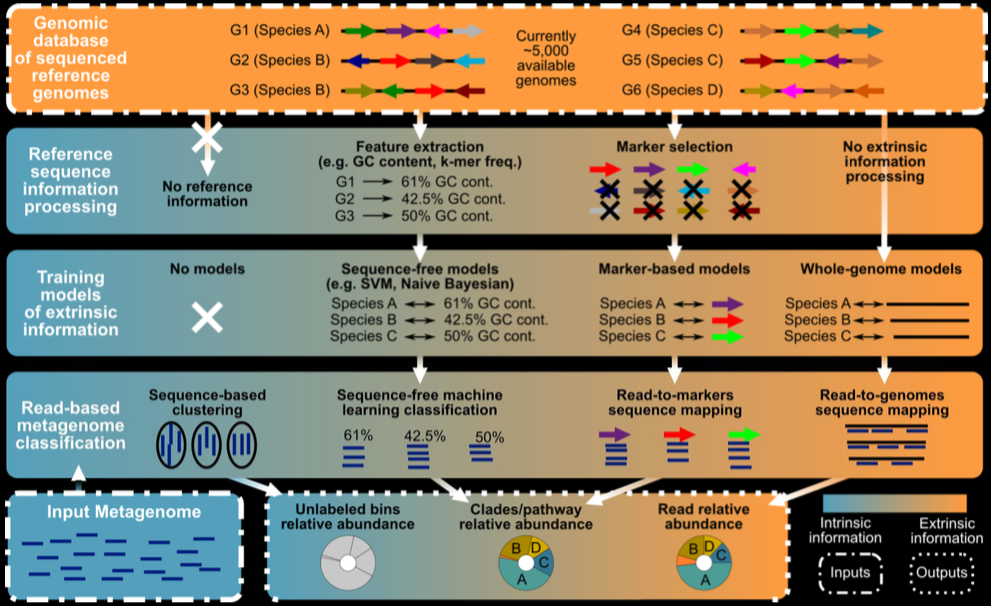
\includegraphics[scale=0.3]{taxApproaches.png}
        \caption{\label{fig:taxApproaches}An overview of taxonomic profiling approaches}
    \end{figure}

    \subsection{The curated MetagenomicData resource}
    Since raw metagenomic sequencing data can be quite difficult to deal with computationally, the curated metagenomic data database stores features obtained from raw metagenomic datasets uniformly processed (MetaPhlAn or HUMAnN2) and integrated with associated metadata obtained from NCBI, papers and authors.
    This database is accessible and can be exploited to perform various types of analysis.

    \begin{figure}[!h]
    \centering
    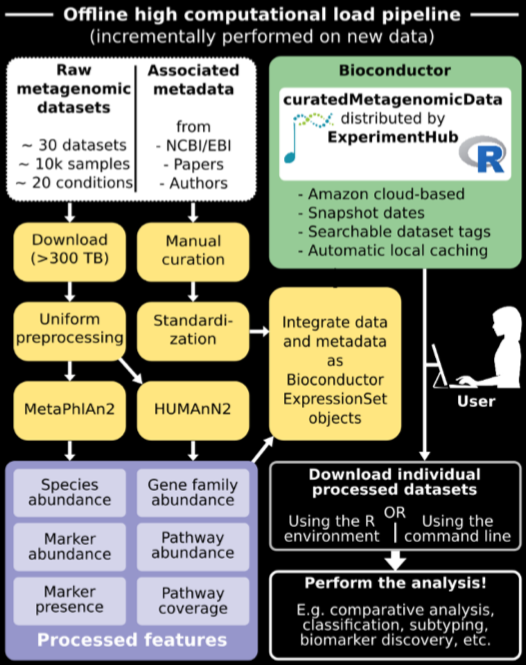
\includegraphics[width=0.4\textwidth]{curatedMetagenomicData.png}
    \caption{\label{fig:curatedMetagenomicData}CuratedMetagenomicData pipeline}
    \end{figure}

    \subsection{The link between the gut microbiome and colorectal cancer}
    Colibactin is a genotoxic metabolite produced by E. coli: it causes damages to the DNA, possibly causing cancer onset.
    A fraction of human colorectal cancer (CRC) cases are caused by colibactin.
    A study published by Segata’s group collected stool samples from people having a colonoscopy in Milan (\ref{fig:milanCRC}) and Turin (\ref{fig:turinCRC}).
    The samples were then categorized after the diagnosis provided by the colonoscopy.
    The aim was the identification of biomarkers associated with the CRC phenotype.
    Different results were obtained in the two cities.

    \begin{figure}[!h]
    \centering
    \begin{subfigure}{.45\textwidth}
        \centering
        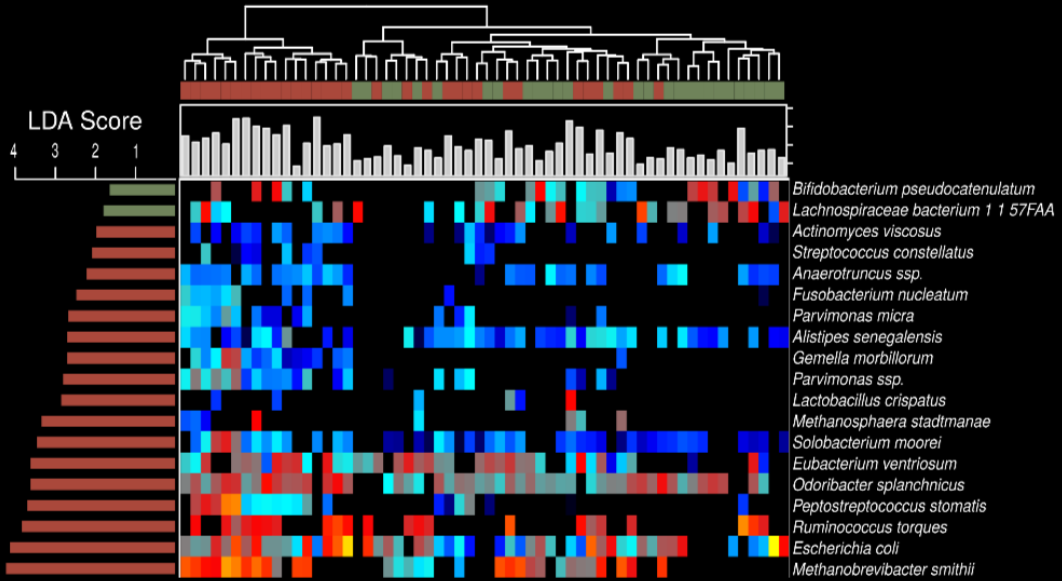
\includegraphics[width=\linewidth]{MilanCRC.png}
        \caption{\label{fig:milanCRC}Patients from Milan}
    \end{subfigure}
    \begin{subfigure}{.45\textwidth}
        \centering
        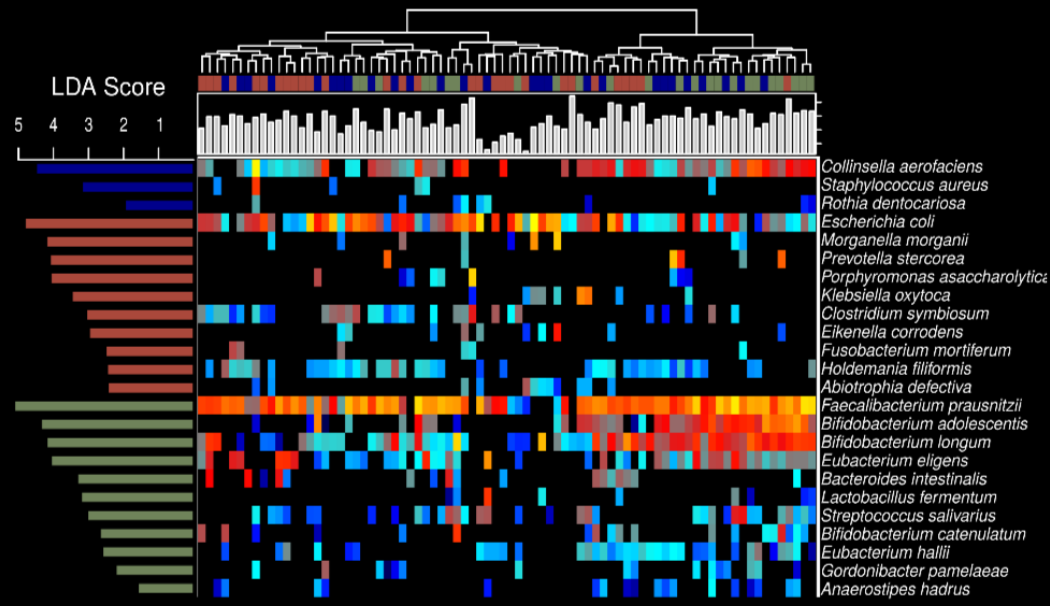
\includegraphics[width=\linewidth]{TurinCRC.png}
        \caption{\label{fig:turinCRC}Patients from Turin}
    \end{subfigure}
    \caption{Taxonomic profiling of gut microbiomes}
    \end{figure}

    Comparing this study with similar ones performed around the world (France, China, Austria, USA, Germany and Japan) some biomarkers appeared to be reproducible (\ref{fig:biomarkers}).
    Moreover, an accuracy around $80\%$ was observed when a machine learning approach (random forest) was applied on all the datasets combined and then the model was applied on a brand new one(\ref{fig:ML}).
    On the other hand, when each group tried the same approach on their data separately, completely different results were found for each dataset, showing that such a technique could be valid for some cases and completely unhelpful for others.

    \begin{figure}[!h]
    \centering
    \begin{subfigure}{.45\textwidth}
        \centering
        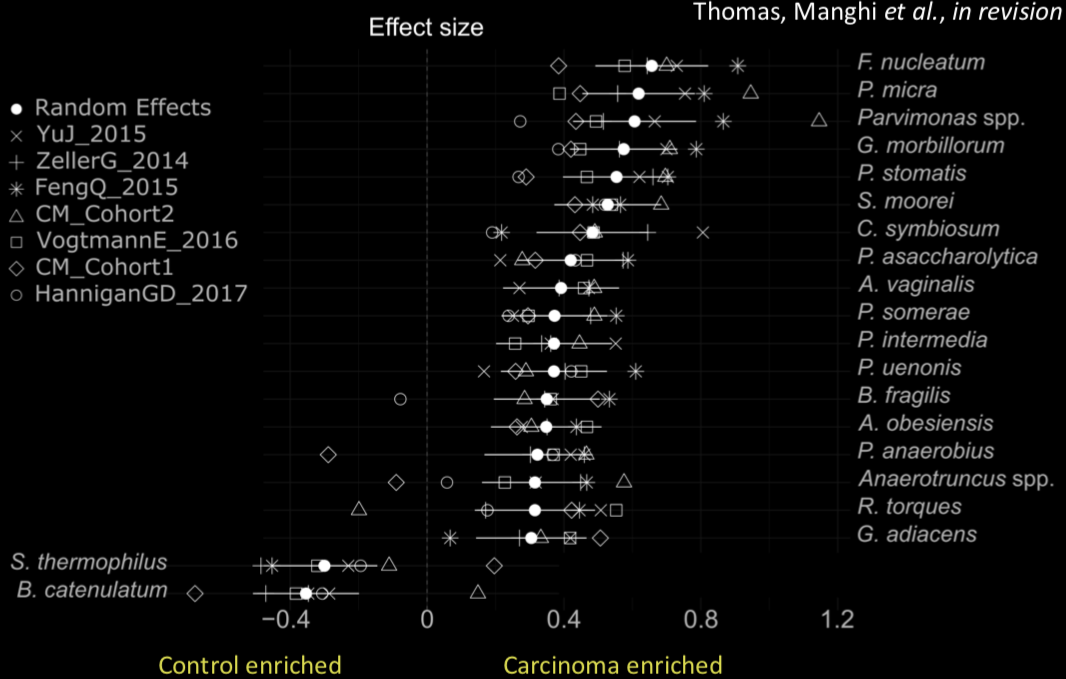
\includegraphics[width=\linewidth]{CRCbiomarkers.png}
        \caption{\label{fig:biomarkers} \emph{F. nucleatum} found to be enriched in datasets with different origins}
    \end{subfigure}
    %
    \begin{subfigure}{.45\textwidth}
        \centering
        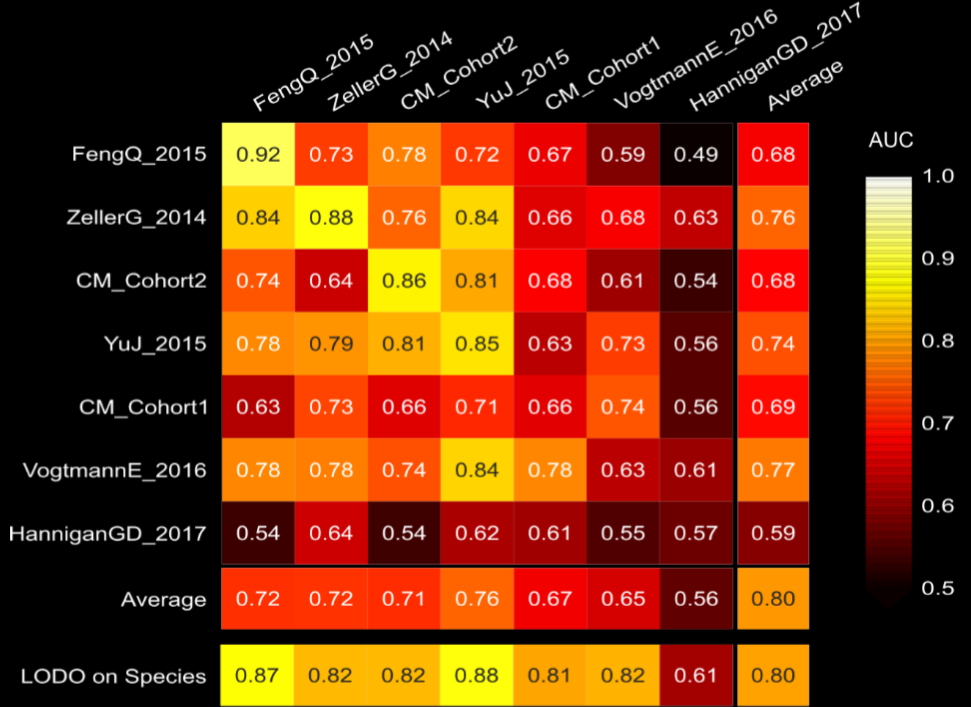
\includegraphics[width=\linewidth]{CRC_ML.png}
        \caption{\label{fig:ML}Random forest approach on all the datasets shows an accuracy of $0.80$ (AUC of $1$ means always right prediction, $0.5$ means no prediction ability)}
    \end{subfigure}
    \caption{}
    \end{figure}


        \subsubsection{Hypothesis-driven analysis}
        The cutC gene appears to be associated with the CRC phenotype (\ref{fig:cutC}).
        The problem is that it is present in several microbial species and it is unknown whether the function and the efficiency are maintained.

        \begin{figure}[H]
            \centering
            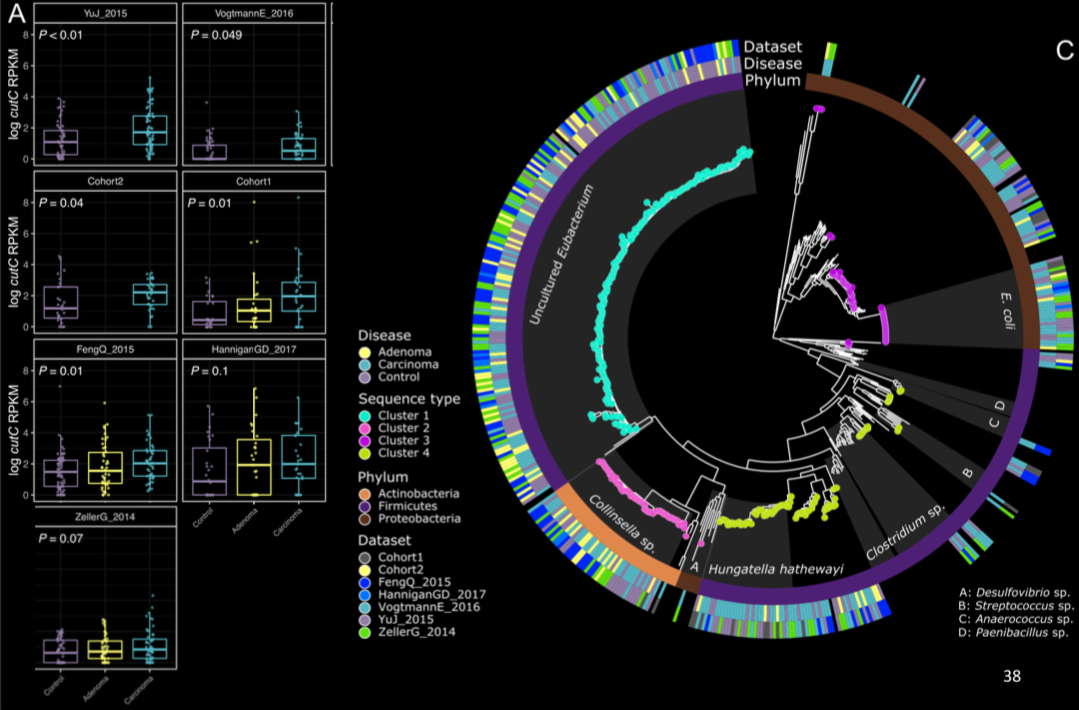
\includegraphics[scale=0.2]{cutC.png}
            \caption{\label{fig:cutC}}
        \end{figure}

    \subsection{PanPhlAn: strain-level profiling}
    PanPhlAn is a tool for strain-level metagenomic profiling that allows to identificate gene composition of individual strains in metagenomic samples.
    The main difficulties to consider with this approach are:

    \begin{multicols}{2}
        \begin{itemize}
            \item Identify the microbial strains present in the metagenome or check whether a specific one is present in the sample.
            \item Discover new strains and species.
            \item Characterize the metagenome genomically.
            \item Track across samples to find the same strain and eventually prove that transmission of bacterial strains occurred among them.
        \end{itemize}
    \end{multicols}

    Let's consider an analysis regarding the \emph{E. coli} pan genome contains about 20.000 gene-families.
    The goal is to find what strains are present in the metagenome and their abundances.
    First all genes are grouped in functional gene-families (\ref{fig:pan1}).
    Then genes from \emph{E. coli} found in the metagenome are mapped on \emph{E. coli} reference genomes with BowTie2.
    The coverage is computed for each gene and then they are grouped into gene-families (\ref{fig:pan2}).
    Then gene-families are ranked based on their coverage.
    Multi-copy gene families have really high coverage, while the plot shows a plateau of single-copy gene-families.
    These families correspond to the strains present in the metagenome and their abundance can be deducted thanks to the base coverage of single-copy genes.

    \begin{figure}[!h]
    \centering
    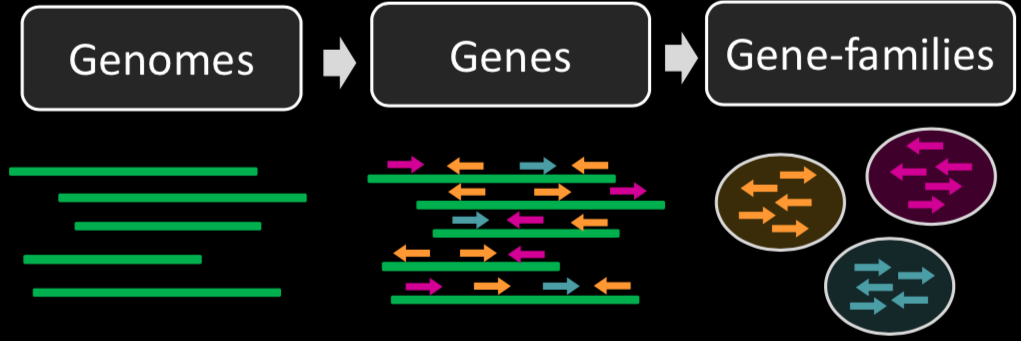
\includegraphics[width=0.9\textwidth]{panphlan1.png}
    \caption{\label{fig:pan1}Genes are grouped in functional gene-families}
    \end{figure}

    \begin{figure}[!h]
    \centering
    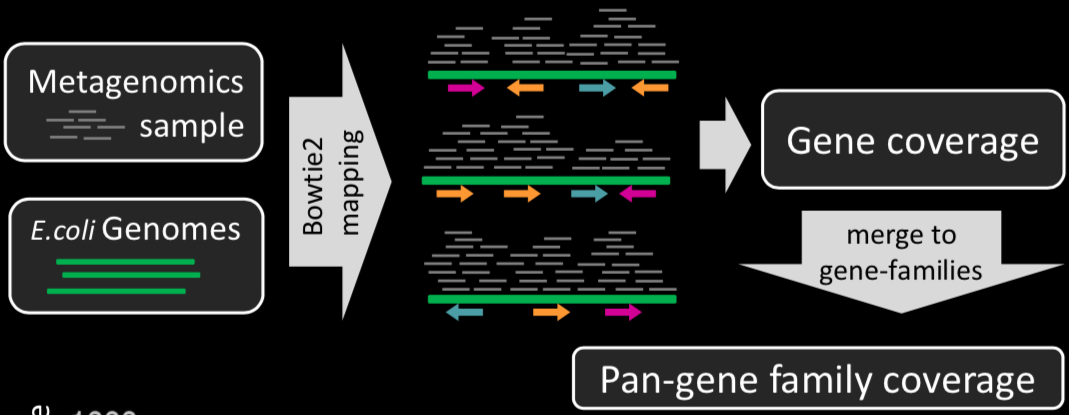
\includegraphics[width=0.9\textwidth]{panphlan2.png}
    \caption{\label{fig:pan2}Mapping and subsequent coverage of gene-families}
    \end{figure}

    \begin{figure}[!h]
    \centering
    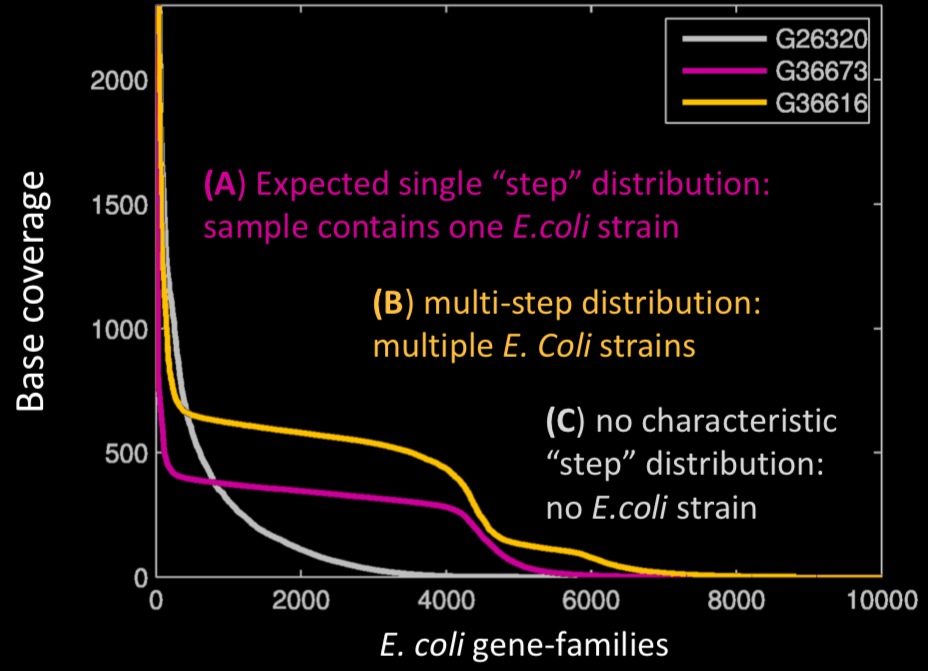
\includegraphics[width=0.6\textwidth]{Coverage.png}
    \caption{\label{fig:pan3}\emph{E. coli} gene-family distribution: curve (A) shows the typical gene-families distribution: multi-copy genes with extremely high coverage, a plateau of single-copy genes and a tail of non-present gene-families. Curves like (C ) should be discarded from the analysis because they indicate that no \emph{E. coli} strain is detected in that sample.}
    \end{figure}

        \subsubsection{Investigating population genomics thanks to PanPhlAn}

            \paragraph{\emph{E. coli} population genomics with PanPhlAn}
            Figure \ref{fig:Ecoli1} shows the \emph{E. coli} profiling of 1478 shotgun metagenomes carried out with PanPhlAn.
            Each column is either an \emph{E. coli} strain obtained via shotgun metagenomics or a reference strain and the columns correspond to the gene-families that can be absent or present in each strain.
            The strains are then clustered (\ref{fig:Ecoli2}) based on which gene-families are present in order to study the population genomics: in this case we can see that the strains isolated from the German \emph{E. coli} outbreak cluster together, while other strains are present in several different areas of the world.

            \begin{figure}[!h]
            \centering
            \begin{subfigure}{.49\textwidth}
                \centering
                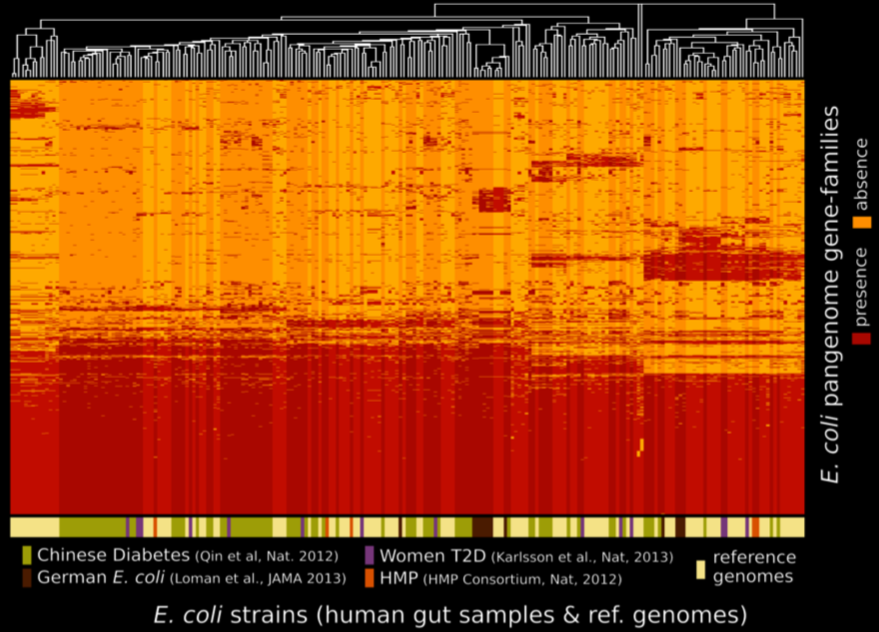
\includegraphics[width=\linewidth]{Ecoli1.png}
                \caption{\label{fig:Ecoli1}}
            \end{subfigure}
            %
            \begin{subfigure}{.49\textwidth}
                \centering
                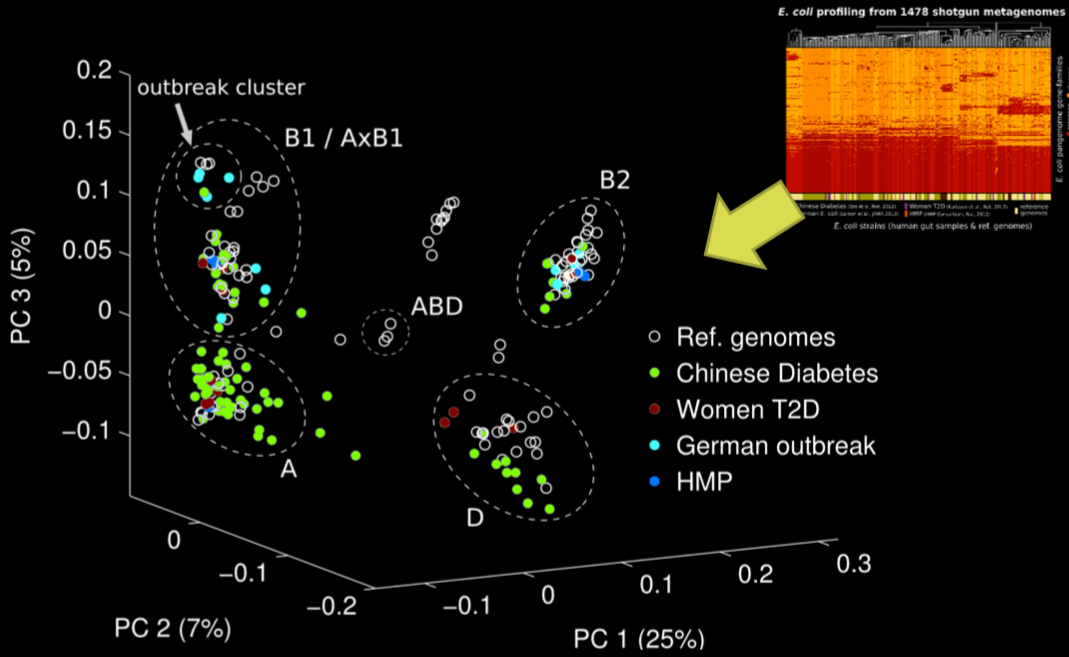
\includegraphics[width=\linewidth]{Ecoli2.png}
                \caption{\label{fig:Ecoli2}}
            \end{subfigure}
            \caption{\emph{E.coli} population genomics with PanPhlAn}
            \end{figure}

            \vspace{2cm}

            \paragraph{PanPhlAn on \emph{Eubacterium rectale}}
            Thanks to PanPhlAn, it was possible to identify many subtypes of \emph{E.rectale} even though only one reference genome was available at the time (\ref{fig:Erec}).

            \begin{figure}[!h]
            \centering
            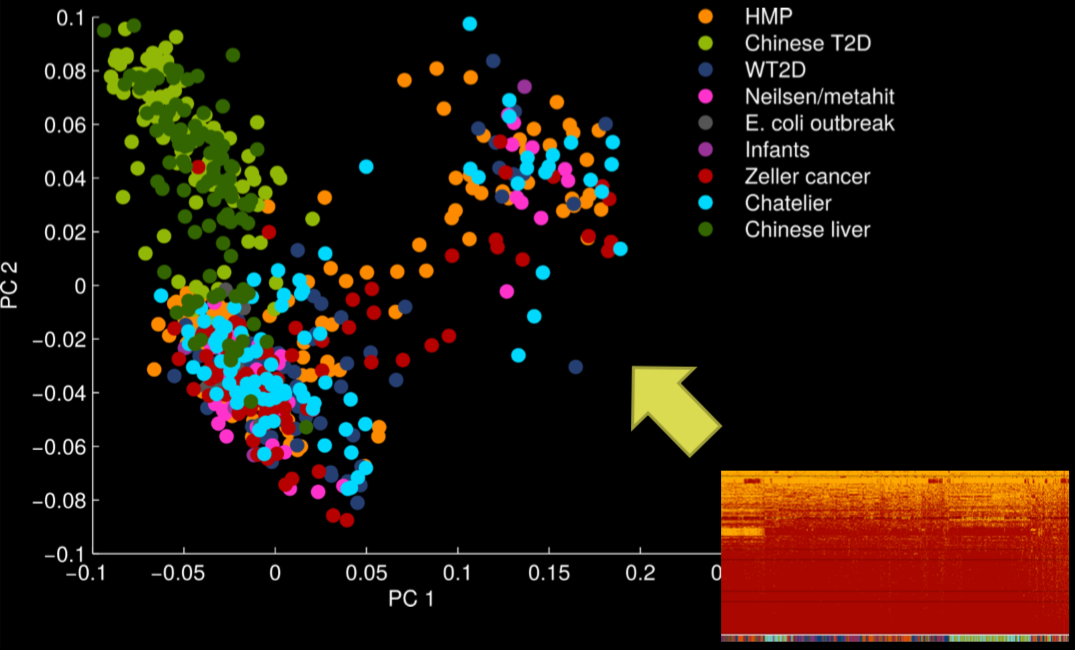
\includegraphics[width=0.6\textwidth]{Erectale.png}
            \caption{\label{fig:Erec} PanPhlAn on \emph{Eubacterium rectale}}
            \end{figure}

            \paragraph{The infant gut microbiome in disease}
            Necrotizing Enterocolitis (NEC) is a devastating disease that affects mostly the intestines of premature infants.
            This study took samples from a cohort of 173 infants, 151 of them were preterm and 30 of them had NEC.
            They obtained 460 shotgun metagenomic samples and 284 shotgun metatranscriptomic samples, all of which were coupled with clinical data of the patients.
            The heatmap shows MetaPhlAn profiling of different bacterial species for all the samples: about 20\% of the patients have a high \emph{E. coli} predominance (\ref{fig:nec1}: yellow circle).
            PanPhlAn was employed to investigate the \emph{E. coli} strains found in these patients: of the 4 identified clades, only 2 are associated with NEC (\ref{fig:nec2}).

            \begin{figure}[!h]
            \centering
            \begin{subfigure}{.45\textwidth}
                \centering
                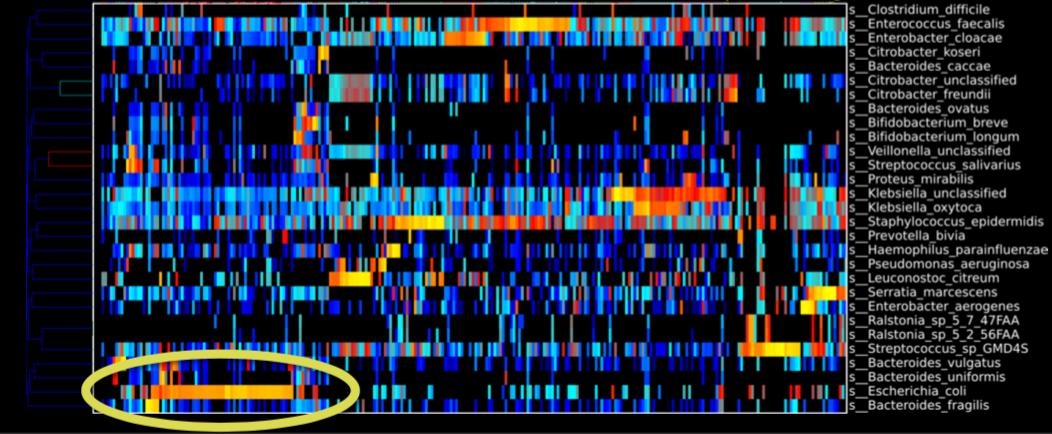
\includegraphics[width=\linewidth]{nec1.png}
                \caption{\label{fig:nec1}MetaPhlAn2 profiling of the cohort of infants}
            \end{subfigure}
            %
            \begin{subfigure}{.45\textwidth}
                \centering
                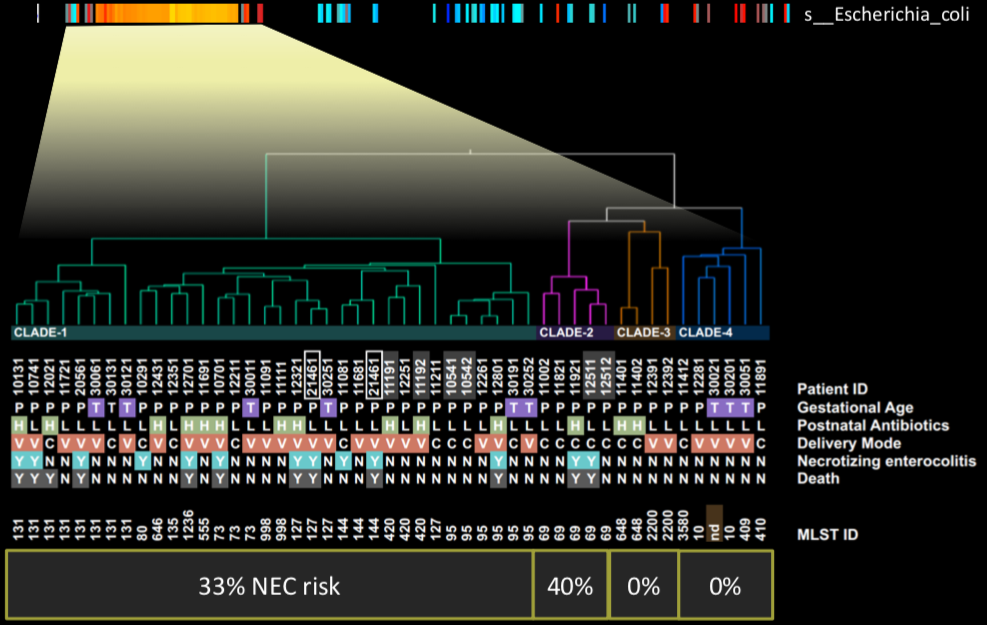
\includegraphics[width=\linewidth]{nec2.png}
                \caption{\label{fig:nec2}PanPhlAn to resolve NEC-assocated E. coli diversity}
            \end{subfigure}
            \caption{The infant gut microbiome in disease}
            \end{figure}

    \subsection{StrainPhlAn}
    The idea in which StrainPhlAn is based on is to base the classification on the genetic variance of core genomes: look for unique combinations of SNPs in genes that are always present and analyse their variance to find some SNPs with a variance different from the others that could characterize a new strain.
    StrainPhlAn exploits MetaPhlAn to compute species-level abundances thanks to species-specific markers and then aligns the marker genes present in the samples to find the SNPs.
    The SNPs are then analysed to build a phylogenetic tree.
    This approach can be applied to many different species.
    For example studies concerning \emph{E. rectale} seems to have a higher resolution compared to the previous approach.

    \begin{figure}[!h]
    \centering
    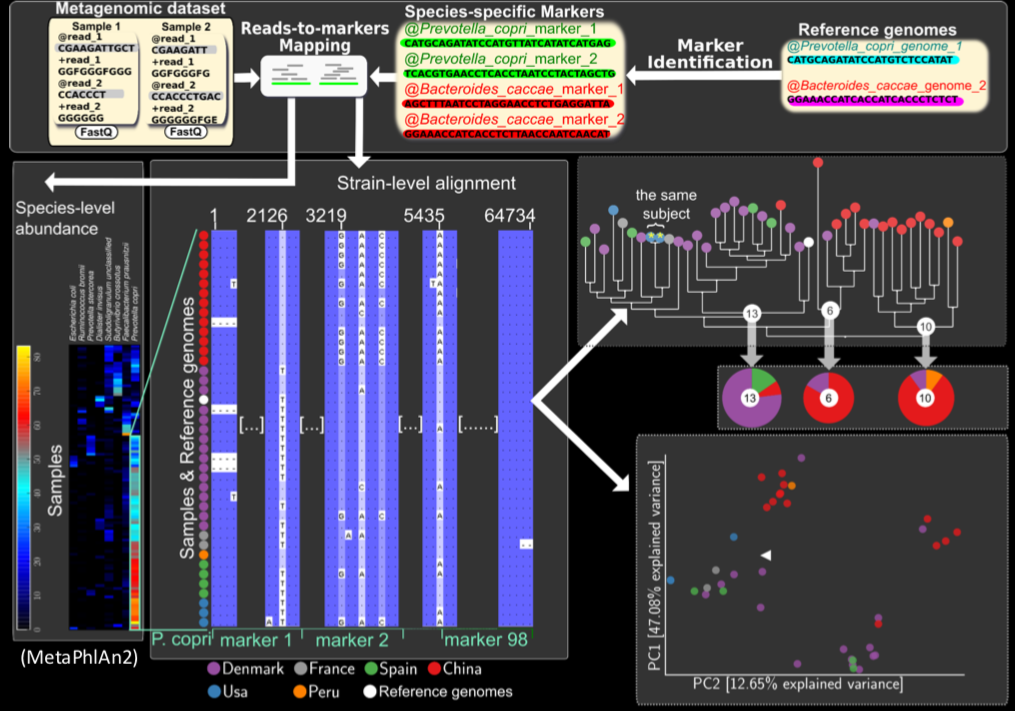
\includegraphics[width=0.9\textwidth]{StrainPhlAn.png}
    \caption{\label{fig:strainphlan}StrainPhlAn pipeline}
    \end{figure}

        \subsubsection{StrainPhlAn applications}

            \paragraph{The stability of strains in the human gut}

            \begin{figure}[!h]
            \centering
            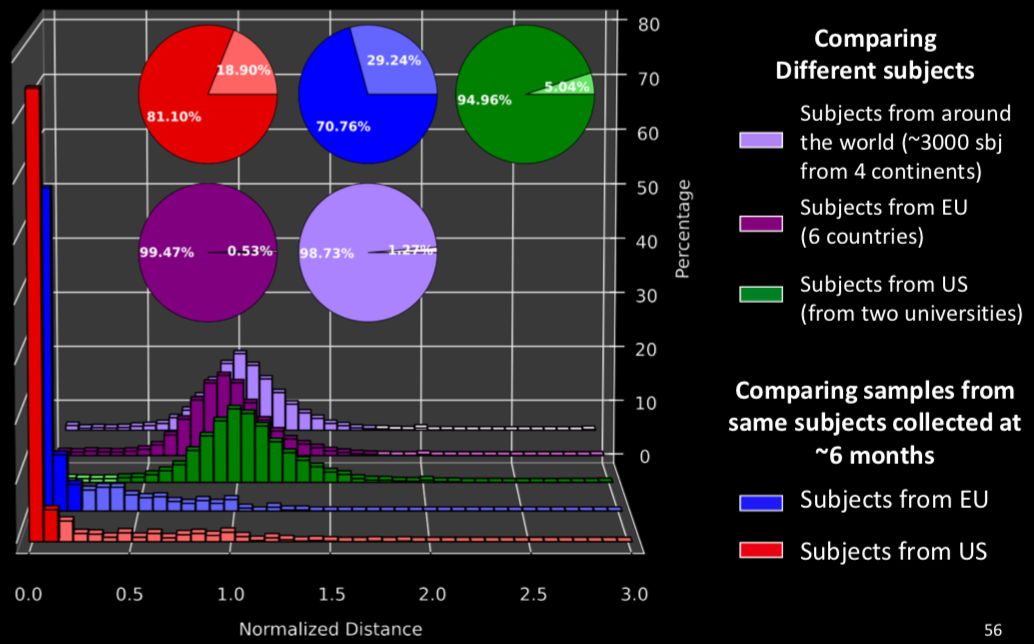
\includegraphics[width=0.8\textwidth]{strainGut.png}
            \caption{\label{fig:gut}The stability of strains in the human gut}
            \end{figure}

            This study analyses samples of the human gut microbiome obtained from different continents.
            The barplots (\ref{fig:gut}) show the distances measured between results of SNPs analysis in different regions around the world.
            There are almost no pairs with zero or low distance and the results do not change if only subjects from the EU or US are considered.
            On the other hand, the red and blue barplots (\ref{fig:gut}) show that comparing the SNPs of samples coming from the same individual but collected 6 months apart they show great similarity.
            This indicates that there is some stability in the human gut microbiome: usually the strains present in one’s gut microbiome tend to remain almost the same.
            Nevertheless, changes of diet or other habits can bring variations in their abundances.

            \paragraph{Identification of subspecies}

            \begin{figure}[!h]
            \centering
            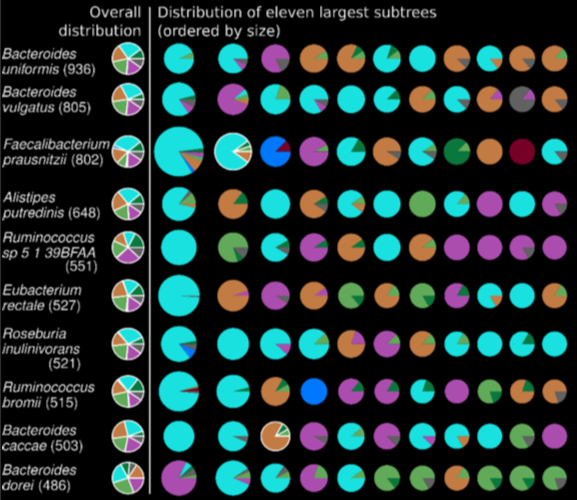
\includegraphics[width=0.5\textwidth]{strainGeo.png}
            \caption{\label{fig:geo}Association of sub-species structures with geography}
            \end{figure}

            Some bacteria are strongly represented in the human population’s microbiomes and their presence is detected in all continents.
            On the other hand subspecies tend to be highly region-specific.
            In Figure \ref{fig:geo}, each color indicates a different country: it is clear that when looking at subspecies of these common microbes, they are mostly associated with only one country or continent.

    \subsection{Uncharacterised species}
    A great amount of information about the human is still unknown:

    \begin{multicols}{2}
        \begin{itemize}
            \item Functional unknowns: genes for which we still do not know the function because they do not match any functional database.
            \item Unknown species/strains: genes not matching any of the known reference genomes.
            \item Undetected unknowns: things we do not know and were not even observed yet.
        \end{itemize}
    \end{multicols}

    \subsection{Workflow for large scale metagenomic assembly}

    Westernized metagenomes are more characterized than non-westernized ones and this study performed a large scale metagenomic assembly on data from undercharacterized region of the world.
    They were able to reconstruct $\sim 70.000$ high quality genomes and $\sim 85.000$ medium-quality ones (with $~50\%$ completeness).

        \subsubsection{Project pipeline}
        Workflow (\ref{fig:workflow2}):

        \begin{multicols}{2}
            \begin{itemize}
                \item Assembly of the reads into contigs.
                \item Binning of contigs into putative genomes (MAGs = Metagenome-Assembled Genomes).
                \item Quality control.
                \item The MAGs are then clustered in species-level genome bins by measuring the distance scores between couples of putative genomes.
                \item SGB are divided into known, unknown and non-human.
            \end{itemize}
        \end{multicols}

        \begin{figure}[h]
        \centering
        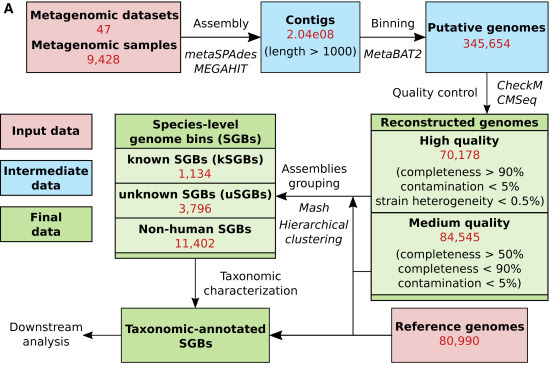
\includegraphics[width=0.9\textwidth]{workflow2.jpg}
        \caption{\label{fig:workflow2}Workflow of large-scale metagenomic assembly}
        \end{figure}

        This study allow to characterize the new cibiobacter.
        In particular Madagascar associated strains of cibiobacter uniquely possess the trp operon for tryptophan metabolism.

\section{Applications of strain-level metagenomic profiling}

    \subsection{\emph{E.rectale} refined population genomics}

    \begin{figure}[!h]
    \centering
    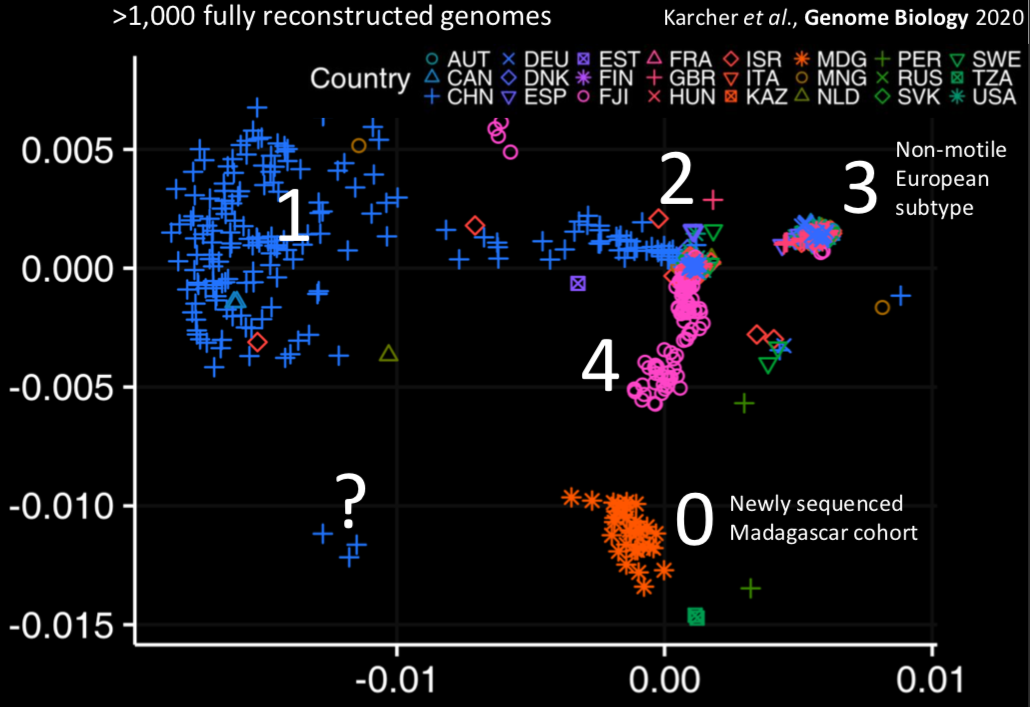
\includegraphics[width=0.8\textwidth]{Erec2.png}
    \caption{\label{fig:Erec2}\emph{E.rectale} refined population genomics}
    \end{figure}

    Thanks to the advancements brought by strain-level metagenomic profiling, a new subtype of \emph{E. rectale} was discovered.
    Subtype 3 lacks the operon coding for motility and other genes that become useless for the bacteria if it is not motile.
    On the other hand, they present more copies of the CAZy genes: these are involved in metabolism and are required by non-motile bacteria in order to be more efficient in the exploitation of carbon sources since they cannot move to reach them.

    \subsection{\emph{Prevotella copri} is strongly lifestyle-associated}

        \begin{figure}[!h]
            \centering
            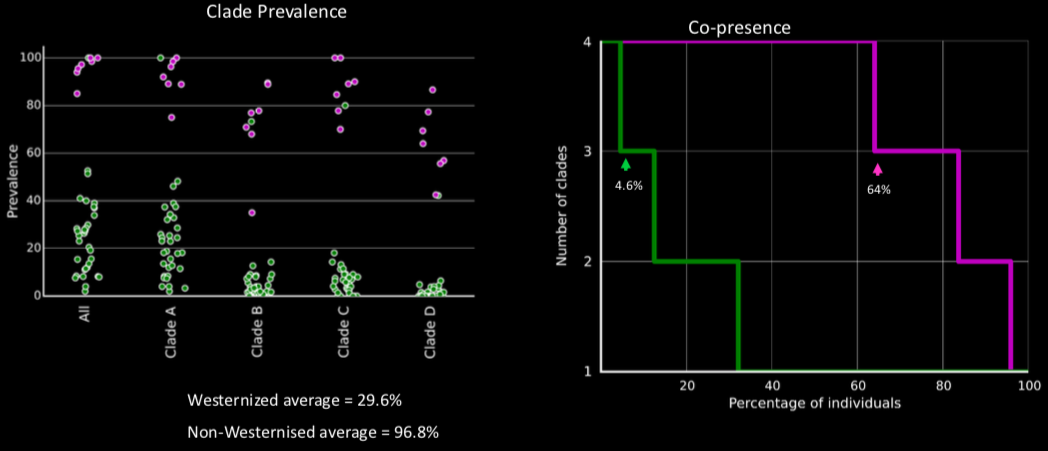
\includegraphics[width=0.8\textwidth]{Prevotella.png}
            \caption{\label{fig:prevotella}\emph{Prevotella copri} is strongly (Western) life-style associated}
        \end{figure}

    \emph{P. copri} is a frequent bacterium in the gut microbiome and it tends to be an on/off one: if it is present, it is the most abundant in the body.
    4 \emph{P. copri} clades with the ability of degrading complex fibers were found.
    They are called clades just because it is not yet confirmed that they can be considered as new strains.
    The interesting part is that westernized populations are associated with a lower prevalence of these clades and with a lower probability of presenting all the $4$ clades together (\ref{fig:prevotella}).
    This is probably caused by our diet: westernized populations tend to eat less complex fibers than non-westernized ones.
    This was confirmed by the analysis of the microbiome found in \"Otzi (3.300 BC) and some ancient Mexican coprolites (600-1300 AD).
    The \emph{P. copri} clades were found in these samples, indicating that we are possibly losing \emph{P. copri} in the westernized populations.

    \subsection{Identification of \emph{Akkermansia} candidate subspecies}
    Only two subspecies of \emph{Akkermansia} have been described and characterized so far: \emph{A. muciniphila} and \emph{A. glycaniphila}.
    In this paper, they used PhyloPhlAn3 to identify 4 MAGs that are candidate \emph{Akkermansia} species.
    Moreover, they observed that these candidate \emph{Akkermansia} species are mutually exclusive for what concerns hosts: they were rarely found coexisting in the same sample.
    They also appear to have different associations in respect to \emph{A. muciniphila}: one is associated with decreased host body mass index (BMI) but the others are not (\ref{fig:akk}).

    \begin{figure}[!h]
        \centering
        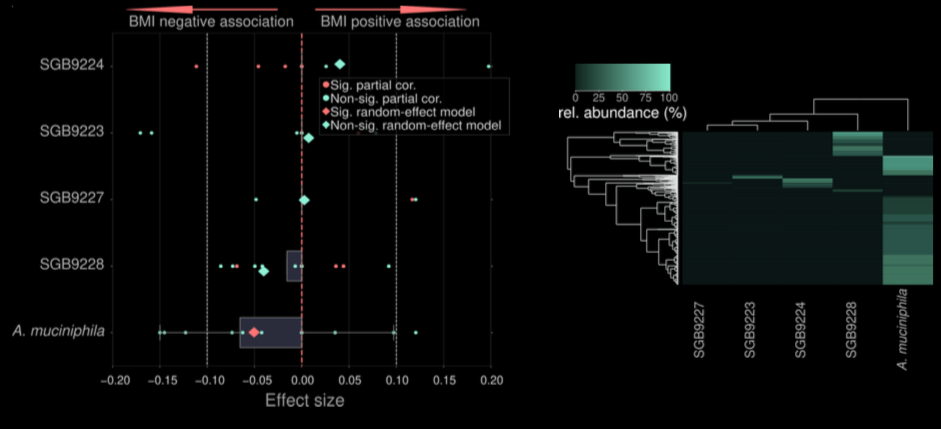
\includegraphics[width=0.8\textwidth]{akkermansia.png}
        \caption{\label{fig:akk}Distinct associations and co-exclusion for the \emph{Akkermansia} (candidate) species}
    \end{figure}

    They also identified putative bacteriophages with spacer hits from \emph{Akkermansia} candidate species and found that viral detectability correlates strongly with the relative abundance of the \emph{Akkermansia} candidate species, suggesting an intimate ecological interplay.
    Analysing \emph{A. muciniphila} subspecies, they determined that these are host-specific: some are found only in mice and some only in humans.

    \subsection{An example of eukaryotic microorganism: \emph{Blastocystis}}
    In this work they developed a pipeline to detect \emph{Blastocystis} subtypes and applied it on 12 large datasets composed of 1689 subjects of different geographic origin, disease status and lifestyle.
    They confirmed that \emph{Blastocystis} is a component of the healthy gut microbiome and found a higher prevalence in non-westernized individuals.
    Moreover, they were able to construct and functionally profile 43 new \emph{Blastocystis} genomes.
    A strong association of specific microbial communities with \emph{Blastocystis} was confirmed by the high predictability of the microorganism colonization based on the species-level composition of the microbiome.

    \subsection{Bacteriophages profiling}

    \begin{figure}[H]
        \centering
        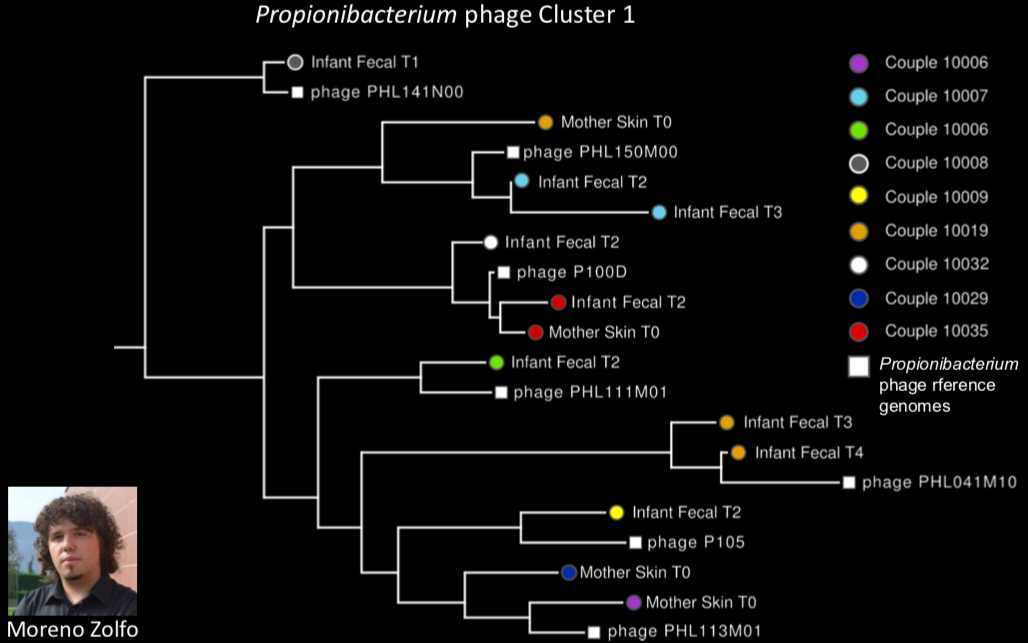
\includegraphics[width=0.8\textwidth]{phages.png}
        \caption{\label{fig:phages}\emph{Propionibacterium} phage Cluster 1}
    \end{figure}

    \subsection{HUMAnN2: Functional profiling}
    The task of mapping nucleotide sequences to proteins that can be done by blastX on a smaller scale is important but computationally challenging.
    Multiple bacteria can be responsible for the same function in the microbiome.
    Thanks to this redundancy, functions are more conserved than bacterial prevalence: the abundance of a bacteria can vary but its function remains efficient because another microbe supplies it.
    For functional profiling, the idea is to reduce the reference dataset by mapping the genes only across proteins that we know are present in the bacteria found in the sample.
    Then the remaining unclassified reads can be mapped to a comprehensive protein database \ref{fig:human2}.

    \begin{figure}[!h]
        \centering
        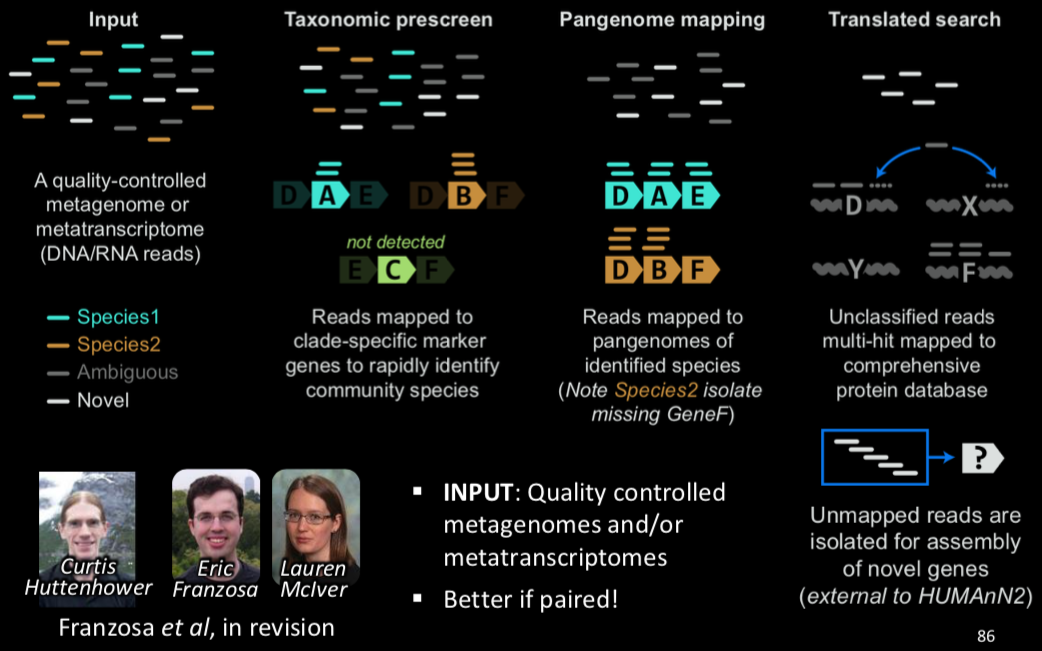
\includegraphics[width=0.8\textwidth]{human2.png}
        \caption{\label{fig:human2}HUMAnN2 workflow}
    \end{figure}
